\documentclass[12pt]{article}
\usepackage[english]{babel}
\usepackage{natbib}
\usepackage{url}
\usepackage[utf8x]{inputenc}
\usepackage{amsmath}
\usepackage{graphicx}
\graphicspath{{images/}}
\usepackage{parskip}
\usepackage{fancyhdr}
\usepackage{subcaption}
\usepackage{relsize}
\usepackage{vmargin}
\setmarginsrb{3 cm}{2.5 cm}{3 cm}{2.5 cm}{1 cm}{1.5 cm}{1 cm}{1.5 cm}

\title{Statistical Pattern Recognition}								% Title
\author{94131091}								% Author
\date{\today}											% Date

\makeatletter
\let\thetitle\@title
\let\theauthor\@author
\let\thedate\@date
\makeatother

\pagestyle{fancy}
\fancyhf{}
\rhead{\theauthor}
\lhead{\thetitle}
\cfoot{\thepage}

\newcommand\numberthis{\addtocounter{equation}{1}\tag{\theequation}}
\newcommand{\gl}{^{>^{w_1}}_{<_{w_2}}}
\newcommand{\svector}[2]{\left[ \begin{matrix} #1 \\ #2 \end{matrix}\right]}
\newcommand{\smatrix}[4]{\left[ \begin{matrix} #1 & #2 \\ #3 & #4 \end{matrix}\right]}
\begin{document}

%%%%%%%%%%%%%%%%%%%%%%%%%%%%%%%%%%%%%%%%%%%%%%%%%%%%%%%%%%%%%%%%%%%%%%%%%%%%%%%%%%%%%%%%%

\begin{titlepage}
	\centering
    \vspace*{0.5 cm}
    
\includegraphics[scale = 1]{Imgs/logo.png}\\[1.0 cm]	% University Logo
    \textsc{\Large Computer Engineering \&\& IT Department\newline\newline Amirkabir University of Technology}\\[2.0 cm]	% University Name
%	\textsc{\large SPR\#1}\\[0.5 cm]				% Course Code
	\rule{\linewidth}{0.2 mm} \\[0.4 cm]
	{ \huge \bfseries \thetitle}\\
	\rule{\linewidth}{0.2 mm} \\[1.5 cm]
	
	\begin{minipage}{0.4\textwidth}
		\begin{flushleft} \large
			\emph{Submitted To:}\\
			Mohammad Rahmati\\
            Asst. Professor\\
            Computer Engineering Department\\
			\end{flushleft}
			\end{minipage}~
			\begin{minipage}{0.4\textwidth}
            
			\begin{flushright} \large
			\emph{Submitted By :} \\
			Ahmad Asadi\\
            94131091\\
            Group-G1\\
            Fall-95\\
		\end{flushright}
        
	\end{minipage}\\[2 cm]
	
	
    
    
    
    
	
\end{titlepage}

%%%%%%%%%%%%%%%%%%%%%%%%%%%%%%%%%%%%%%%%%%%%%%%%%%%%%%%%%%%%%%%%%%%%%%%%%%%%%%%%%%%%%%%%%

\tableofcontents
\pagebreak

%%%%%%%%%%%%%%%%%%%%%%%%%%%%%%%%%%%%%%%%%%%%%%%%%%%%%%%%%%%%%%%%%%%%%%%%%%%%%%%%%%%%%%%%%

\section{Problem 1}
Two normal distribution are characterized by: 
\begin{align*}
&P_1 = P_2 = 0.5 \\
&M_1 = \left[ \begin{matrix}
1 \\ 
0 
\end{matrix} 
\right] \> \> \> \>
\Sigma_1 = \left[
\begin{matrix}
1 & 0.5 \\
0.5 & 1
\end{matrix}
\right] \\
&M_2 = \left[ \begin{matrix}
-1 \\ 
0 
\end{matrix} 
\right] \> \> \> \>
\Sigma_2 = \left[
\begin{matrix}
1 & -0.5 \\
-0.5 & 1
\end{matrix}
\right]
\end{align*}
\begin{enumerate}
\item Draw the Bayes decision boundary to minimize the probability of error. \\

The bayesian decision function is:\\
\begin{align*}
&P(X | w_1) \cdot P(w_1)^{>^{w_1}}_{<_{w_2}}  P(X | w_2) \cdot P(w_2) \\
&\frac{P(X | w_1) \cdot P(w_1)}{P(X | w_2) \cdot P(w_2)} .^{>^{w_1}}_{<_{w_2}} 1\rightarrow\frac{P(X | w_1)}{P(X | w_2)} .^{>^{w_1}}_{<_{w_2}} 1
\end{align*}
The figure \ref{fig:1} displays the data distributions and decision boundaries of bayesian decision function without considering costs.

\begin{figure}[h]
\centering
\begin{subfigure}{0.35\textwidth}
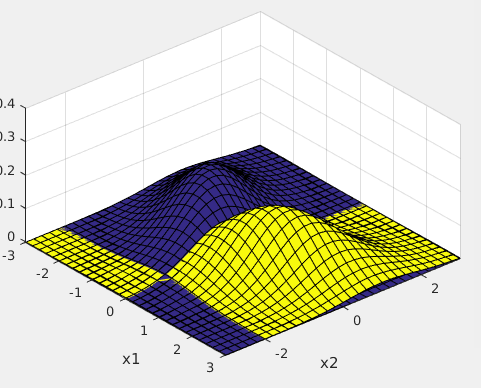
\includegraphics[scale=0.3]{Imgs/hw1-1-1.png}
\caption{Distribution of data. The distribution of class 1 is displayed in blue color and the distribution of class 2 is displayed in yellow.}
\end{subfigure}
\begin{subfigure}{0.35\textwidth}
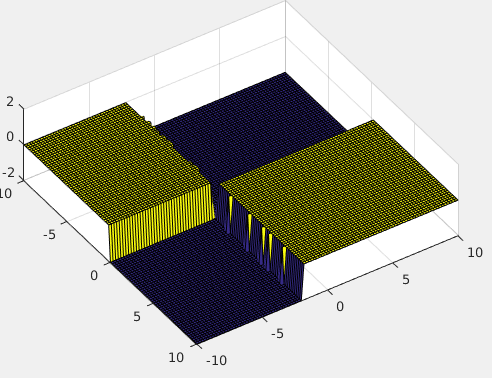
\includegraphics[scale=0.3]{Imgs/hw1-1-2.png}
\caption{Decision Boundary. The decision boundary of class 1 is displayed in blue color and the that of class 2 is displayed in yellow.}
\end{subfigure}
\caption{Bayesian Decision Boundary without considering decision costs}
\label{fig:1}
\end{figure}

Also, it is possible to transform the data to a one dimensional space first and make decision in the new space using a single threshold as bellow:

\begin{align*}
h(X) = &\frac{1}{2}(X-M_1)^T\Sigma_1^{-1}(X-M_1) - \frac{1}{2}(X-M_2)^T\Sigma_2^{-1}(X-M_2) \\
& + \frac{1}{2}ln\frac{|\Sigma_1|}{|\Sigma_2|} .\gl ln \frac{P(W_1)}{P(W_2)} \\
&\rightarrow h(X) = \frac{1}{2}(X-\svector{1}{0})^T\smatrix{1}{0.5}{0.5}{1}^{-1}(X-\svector{1}{0}) \\
&- \frac{1}{2}(X-\svector{-1}{0})^T\smatrix{1}{-0.5}{-0.5}{1}^{-1}(X-\svector{-1}{0}) \\
&+ \frac{1}{2}ln\frac{|\smatrix{1}{0.5}{0.5}{1}|}{|\smatrix{1}{-0.5}{-0.5}{1}|} .\gl 0 \\
&\rightarrow h(X) = \frac{1}{2}(X-\svector{1}{0})^T\smatrix{1}{0.5}{0.5}{1}^{-1}(X-\svector{1}{0}) \\
&- \frac{1}{2}(X-\svector{-1}{0})^T\smatrix{1}{-0.5}{-0.5}{1}^{-1}(X-\svector{-1}{0}) .\gl 0
\end{align*}

\begin{center}
\line(1,0){250}
\end{center}

%%%%%%%%%%%%%%%%%%%%%%%%%%%%%%%%%%%
\item Draw the Bayes decision boundary to minimize the cost with $c_{11} = c_{22} = 0$ and
$c_{12} = 2c_{21}$ \\
The Bayesian decision boundary when considering costs of decisions turns to the form bellow:
\begin{equation}
\mathlarger{\frac{p_1(X)}{p_2(X)}} .^{>^{w_1}}_{<_{w_2}} \mathlarger{\frac{(c_{12} - c_{22})P_2}{(c_{21} - c_{11})P_1}}
\label{eq:1-1}
\end{equation}
Figure \ref{fig:1-2} displays the decision boundary in this case.


\begin{figure}[h]
\centering
\begin{subfigure}{0.4\textwidth}
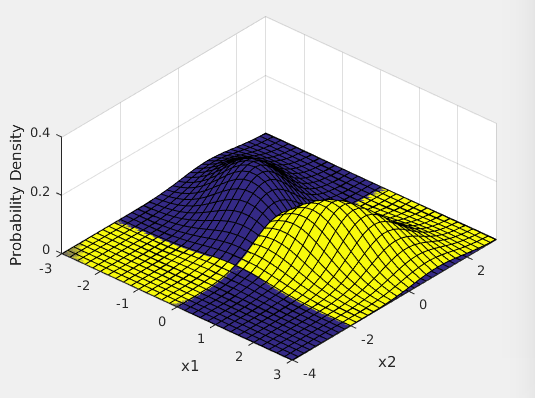
\includegraphics[scale=0.3]{Imgs/1-2-1.png}
\caption{Distribution of data. The distribution of class 1 is displayed in yellow color and the distribution of class 2 is displayed in blue.}
\end{subfigure}
\begin{subfigure}{0.4\textwidth}
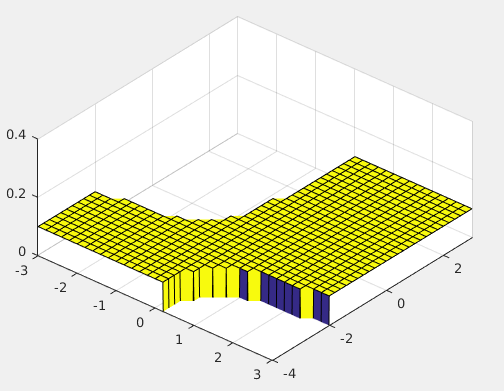
\includegraphics[scale=0.3]{Imgs/1-2-2.png}
\caption{Decision Boundary. The decision boundary of class 1 is displayed in yellow color and the that of class 2 is displayed in blue.}
\end{subfigure}
\caption{Bayesian Decision Boundary considering decision costs $c_{11} = c_{22} = 0$ and $c_12 = 2c_{21}$}
\label{fig:1-2}
\end{figure}

\begin{center}
\line(1,0){250}
\end{center}

%%%%%%%%%%%%%%%%%%%%%%%%%%%%%%%%%%%
\item Assume that $c_{11} = c_{22} = 0$ and $c_{12} = c_{21}$ :
\begin{enumerate}

\item Plot the operating characteristics.

As equation \eqref{eq:1-1} yields, with $c_{11} = c_{22} = 0$ and $c_{12} = c_{21}$ the decision boundary is not different from that of section 1. So the figure \ref{fig:1} is displaying the required decision boundary

\begin{center}
\line(1,0){250}
\end{center}

%%%%%%%%%%%%%%%%%%%%%%%%%%%%%%%%%%%
\item Find the total error when Neyman-Pearson test is performed with $\epsilon_1 = 0.05$ \\

We should estimate $\mu$ such that the following function $r$ be minimized.
\begin{equation}
r = \mu(\epsilon_1 - 0.05) + \epsilon_2
\end{equation}
After finding appropriate $\mu$, the decision boundary is derivable from:
\begin{equation}
\mathlarger{\frac{p_1(X)}{p_2(X)}} .\gl \mu
\end{equation}
To find such $\mu$ an script will iterate on following equation to reach the best fitting value.
\begin{equation}
\epsilon_1 = \int^{\infty}_\mu p_h(h|W-1) dh = 0.05
\end{equation}

The $\mu = 1.0795e-78$ is the best value estimated with $\epsilon_1 = 0.051$ error rate. Figure \ref{fig:1-3} illustrates the resulted decision boundary.

\begin{figure}[h]
\centering
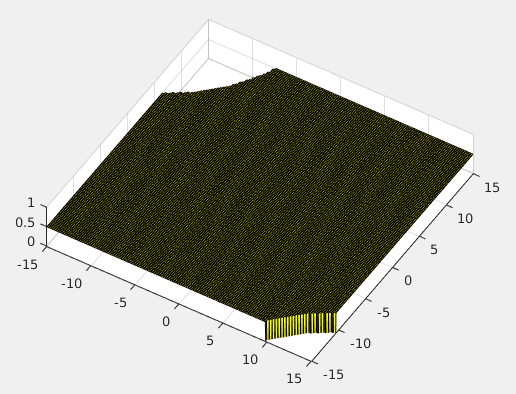
\includegraphics[scale=0.4]{Imgs/1-3-1.png}
\caption{Decision boundary resulted from Neyman-Pearson test with $\epsilon_1 = 0.05$}
\label{fig:1-3}

\end{figure}

\begin{center}
\line(1,0){250}
\end{center}

%%%%%%%%%%%%%%%%%%%%%%%%%%%%%%%%%%%
\item Find the threshold value and total error for the minimax test.

\begin{center}
\line(1,0){250}
\end{center}

%%%%%%%%%%%%%%%%%%%%%%%%%%%%%%%%%%%
\item Plot the error-reject curve.

\end{enumerate} 
\end{enumerate}


\begin{center}
\line(1,0){450}
\end{center}



%%%%%%%%%%%%%%%%%%%%%%%%%%%%%%%%%%%%%%%%%%%%%%%%%%%%%%%%%%%%%%%%%%%%%%%%%%%%%%%%%%%%%%%%%

\section{Problem 2}
Two normal distribution are characterized by: 
\begin{align*}
&P_1 = P_2 = 0.5 \\
&M_1 = \left[ \begin{matrix}
1 \\ 
0 
\end{matrix} 
\right] \> \> \> \>
\Sigma_1 = \left[
\begin{matrix}
4 & -3 \\
-3 & 4
\end{matrix}
\right] \\
&M_2 = \left[ \begin{matrix}
-1 \\ 
0 
\end{matrix} 
\right] \> \> \> \>
\Sigma_2 = \left[
\begin{matrix}
4 & 3 \\
3 & 4
\end{matrix}
\right]
\end{align*}
\begin{enumerate}
\item Find the linear discriminant function which maximize the Fisher criterion and
minimize the error by adjusting the threshold.\\
\begin{align*}
&f = \mathlarger{\frac{(\mu_1 - \mu_2)^2}{\sigma_1^2 + \sigma_2^2}} \rightarrow \frac{\partial f}{\partial \sigma_1^2} =  \frac{\partial f}{\partial \sigma_2^2} = \mathlarger{\frac{-(\mu_1 - \mu_2)^2}{(\sigma_1^2 + \sigma_2^2)^2}} \\
&\rightarrow s = \mathlarger{\mathlarger{\frac{\frac{\partial f}{\partial \sigma_1^2}}{\frac{\partial f}{\partial \sigma_1^2} + \frac{\partial f}{\partial \sigma_2^2}}}} = 0.5\\
&\rightarrow V = [0.5 \Sigma_1 + 0.5 \Sigma_2]^-1 (\mu_1 - \mu_2) = \left[\begin{matrix}
4 & 0\\
0 & 4
\end{matrix}
\right]^-1 \left[ \begin{matrix}
-2 \\
0
\end{matrix} \right] = \frac{1}{16} \left[ \begin{matrix}
4 & 0 \\
0 & 4
\end{matrix} \right] \left[ \begin{matrix}
-2 \\
0
\end{matrix} \right] \\ 
&\rightarrow V = \left[ \begin{matrix}
-0.5\\0
\end{matrix}\right] \numberthis \label{eq:1}
\end{align*}
Equation \eqref{eq:1} illustrates the best mapping vector $V$ to project distribution over, therefore the LDA will be in the form of $V^t x \geq \alpha$, in which $\alpha$ should be find from equation \eqref{eq:2}.
\begin{equation}
\frac{\partial f}{\partial \mu_1} + \frac{\partial f}{\partial \mu_2} = 0
\label{eq:2}
\end{equation}
which results:
\begin{align*}
&\frac{2\mu_1 - 2\mu_2}{\sigma_1^2 + \sigma_2^2} + \frac{- 2\mu_1 + 2\mu_2}{\sigma_1^2 + \sigma_2^2} = 0 \rightarrow 0 = 0
\end{align*}
Therefore, the best $\alpha$ is not derivable analytical. In order to estimate the best $\alpha$ a MATLAB script using bootstrapping has been written by me, which is appended to the homework submission zip file. The bootstrapping process, iterates 1000 number of times in each iteration generating 1000 multivariate random variables regarding given means and variances for each class. We attempt to estimate best $\alpha$ in each iteration using grid search in the range of $[-4,4]$ with step length 0.01. To measure the accuracy of chosen $\alpha$ we use the ratio $\frac{tp + tn - fp - fn}{N}$ as the measurement function. After all iterations, the mean of all best estimated $\alpha$s is reported as the best $\alpha$. Experiments resulted the $\alpha = 0.23$ as the best value separating two classes from each other. So the LDA function is being reformed as bellow:
\begin{equation}
\left[ \begin{matrix}
-0.5 \\ 0
\end{matrix} \right]^T X \geq^{w_1} 0.23
\end{equation}
\begin{center}
\line(1,0){250}
\end{center}

\item Find the optimum linear discriminant function which minimize the probability of
error.\\
The iterative process has been coded in MATLAB and its code is attached to the submitted homework zip file. \\
The parameter $s$ has been estimated using a grid search in rage $[0, 1]$ with step length 0.01. the error probability $epsilon$ in each iteration with respect to selected $s$ has been calculated. The figure \ref{fig:2} illustrates the behaviour of error probability w.r.t. selected $s$. The best value of $s$ is in 0 or 1. 

\begin{figure}[h]
\centering
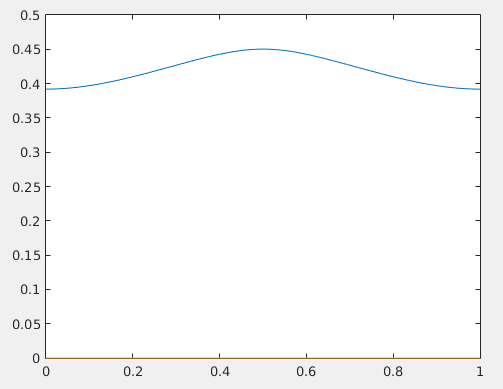
\includegraphics[scale=0.4]{Imgs/2_2_1.png}
\caption{The behaviour of error probability $\epsilon$ w.r.t. chosen $s$}
\label{fig:2}
\end{figure}

\begin{figure}[h]
\centering
\begin{subfigure}{0.4\textwidth}
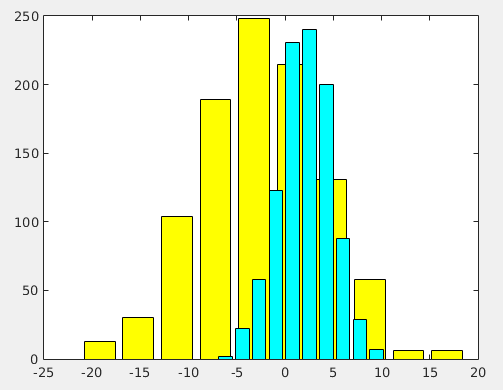
\includegraphics[scale=0.3]{Imgs/2_2_2.png}
\caption{Projected distribution of data. The projected distribution of class 1 w.r.t. mapping vector $V$ is displayed in blue color and the that of class 2 is displayed in yellow when $s = 1$ (BEST CASE).}
\end{subfigure}
\begin{subfigure}{0.4\textwidth}
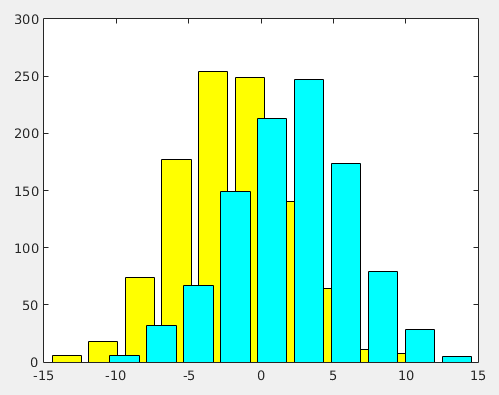
\includegraphics[scale=0.3]{Imgs/2_2_3.png}
\caption{Projected distribution of data. The projected distribution of class 1 w.r.t. mapping vector $V$ is displayed in blue color and the that of class 2 is displayed in yellow when $s = 0.5$ (WORST CASE).}
\end{subfigure}
\caption{A comparison between projected distributions over matrices $V$ w.r.t. selected $s$}
\label{fig:3}
\end{figure}


To through a light over reality, the projection of data in two cases of $s = 0.5$ and $s = 1$ has been displayed in the figure \ref{fig:3}, respectively the worst- and the best-case. As its obviously clear, the separation of classes is more suitable in case $s = 1$ rather than $s = 0.5$, hence the lower error probability will be gained when $s = 1$.



\end{enumerate}

\begin{center}
\line(1,0){450}
\end{center}

%%%%%%%%%%%%%%%%%%%%%%%%%%%%%%%%%%%%%%%%%%%%%%%%%%%%%%%%%%%%%%%%%%%%%%%%%%%%%%%%%%%%%%%%
\section{Problem 3}
We consider a classification problem in dimension $d=2$, with $k=3$ classes where:
$p ( x | w_i ) \propto N ( \mu_i , \Sigma_i ), i = 1 , 2 , 3 , $ with:
\begin{align*}
\mu_1 = \left[ \begin{matrix}
0 \\ 2
\end{matrix} \right] ,
\mu_2 = \left[ \begin{matrix}
3 \\ 1
\end{matrix} \right] ,
\mu_3 = \left[ \begin{matrix}
1 \\ 0
\end{matrix} \right] ,
\Sigma_i = \Sigma = \left[ \begin{matrix}
1 & 0 \\
0 & \frac{1}{3}
\end{matrix} \right]
\end{align*}
\begin{enumerate}
\item Calculate the discriminant function $g_i(x)$ for each class. \\
Generating a discriminant function between all pairs of classes can be a good solution. Assuming $P(W_1)=P(W_2)=P(W_3)$, the Bayes classifier is a good choice:
\begin{align*}
d_{ij}: \mathlarger{\frac{P(X|W_i)}{P(X|W_j)}}.^{>^{W_i}}_{<_{W_j}} 1
\end{align*}
Defining such classifiers, the feature function $g_i(X)$ can be defined as :
\begin{align*}
&g_1(X) = \Pi_{j=2,3}sgn(\frac{P(X|W_1)}{P(X|W_j)} - 1) \\
&g_2(X) = \Pi_{j=2,3}sgn(\frac{P(X|W_2)}{P(X|W_j)} - 1) \\
&g_3(X) = \Pi_{j=2,3}sgn(\frac{P(X|W_3)}{P(X|W_j)} - 1) \\
\end{align*}
In which the positive value of each function $g_i(X)$ indicates that $X$ belongs to $W_i$ and vice versa. 

\begin{center}
\line(1,0){250}
\end{center}

%%%%%%%%%%%%%%%%%%%%%%%%%%%%%%%%%%%
\item Express your discriminant functions in the form of linear discriminant functions. \\
The $d_{ij}$s could be expressed as linear functions as perpendicular bisectors of linking line between the center points of each class:
\begin{align*}
&d_{12} = X_2 + 3X_1 + 3 \\
&d_{13} = X_2 + \frac{1}{2}X_1 - \frac{3}{4} \\
&d_{23} = X_2 + 2X_1 - \frac{9}{2} \\
\end{align*}
Defining $d_{ij}(X) = -d_{ji}(X)$, the vector $X$ belongs to class $W_i$ iff $ \forall j \neq i , d_{ij}(X) > 0 $

\begin{center}
\line(1,0){250}
\end{center}

%%%%%%%%%%%%%%%%%%%%%%%%%%%%%%%%%%%
\item Determine and plot the decision boundaries.
Figure \ref{fig:3-1} displays the distribution of data given mean vectors and covariance matrices.
\begin{figure}[h]
\centering
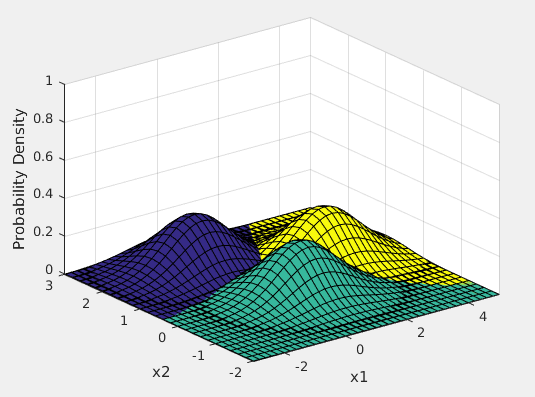
\includegraphics[scale=0.5]{Imgs/3-1.png}
\caption{Data distribution w.r.t. means and covariance matrices}
\label{fig:3-1}
\end{figure}

Figure \ref{fig:3-2} displays the data distribution boundary and deriven boundaries using two-class discriminant functions defined in section 2 of this problem.


\begin{figure}[h]
\centering
\begin{subfigure}{0.4\textwidth}
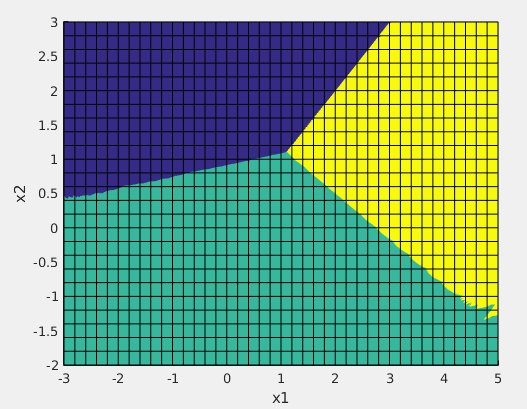
\includegraphics[scale=0.3]{Imgs/3-2.png}
\caption{Projected distribution of data on $X1-X2$ coordinates}
\end{subfigure}
\begin{subfigure}{0.4\textwidth}
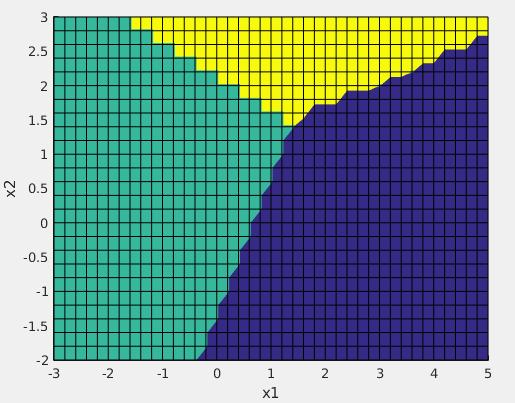
\includegraphics[scale=0.3]{Imgs/3-3.png}
\caption{Boundaries generated by discriminant functions}
\end{subfigure}
\caption{A comparison between projected distributions over matrices $V$ w.r.t. selected $s$}
\label{fig:3-2}
\end{figure}


\begin{center}
\line(1,0){450}
\end{center}



\end{enumerate}

%%%%%%%%%%%%%%%%%%%%%%%%%%%%%%%%%%%%%%%%%%%%%%%%%%%%%%%%%%%%%%5%%%%%%%%%%%%%%%%%%%%%%%%%%%%%%%%%%%
\section{Problem 4}
Consider the following 2-class classification problem involving a single feature $x$.
Assume equal class priors and 0-1 loss function.
\begin{center}
$
p(x|w_1) = \left\lbrace \begin{matrix}
2x & 0 \leq x \leq 1 \\
0 & otherwise
\end{matrix} \right\rbrace,
p(x|w_2) = \left\lbrace \begin{matrix}
2 - 2x & 0 \leq x \leq 1 \\
0 & otherwise
\end{matrix} \right\rbrace,
$
\end{center}

\begin{enumerate}
\item Sketch the two densities
Since the class priors are equal:
\begin{align*}
&p(w_1 | x) = \mathlarger{\frac{p(x|w_1) p(w_1)}{\Sigma_{i=1}^2p(x|w_i) p(w_i)}} = \frac{0.5(2x)}{1} = x\\
&p(w_2 | x) = \mathlarger{\frac{p(x|w_2) p(w_2)}{\Sigma_{i=1}^2p(x|w_i) p(w_i)}} = \frac{0.5(2 - 2x)}{1} = 1 - x\\
\end{align*}

\begin{center}
\line(1,0){250}
\end{center}

%%%%%%%%%%%%%%%%%%%%%%%%%%%%%%%%%%%
\item State the Bayes decision rule and show the decision boundary.

\begin{align*}
&p(w_1|x)\gl p(w_2|x) \rightarrow x\gl 1-x \rightarrow 2x - 1\gl 0
\end{align*}

Figure \ref{fig:4-1} displays the data distribution, decision boundary, false positive and false negative errors. The area coloured blue and green are displaying correct classifications for class $w_1$ and $w_2$ respectively. The yellow and red areas are illustrating $\epsilon_1$ and $\epsilon_2$ respectively.

\begin{figure}[h]
\centering
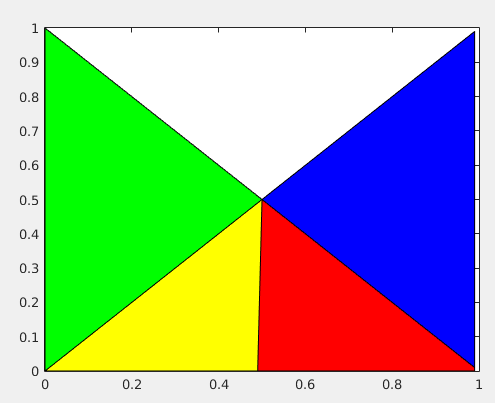
\includegraphics[scale=0.4]{Imgs/4-1.png}
\caption{Bayes decision boundary for proposed data in problem 4 when $p(w_1) = p(w_2) = 0.5$}
\label{fig:4-1}
\end{figure}



\begin{center}
\line(1,0){250}
\end{center}

%%%%%%%%%%%%%%%%%%%%%%%%%%%%%%%%%%%
\item What is the Bayes classification error?
The classification error is being calculated as a weighted sum of each misclassified point w.r.t. its probability. Therefore,
\begin{align*}
\epsilon = 0.5 * \epsilon_1 + 0.5 * \epsilon_2 = 0.5 * \int_0^0.5 x dx + 0.5 * \int_0.5^1 1-x dx = \frac{1}{16} + \frac{1}{16}  = \frac{1}{8}
\end{align*}
\begin{center}
\line(1,0){250}
\end{center}

%%%%%%%%%%%%%%%%%%%%%%%%%%%%%%%%%%%
\item How will the decision boundary change if the prior for class $w_2$ is increased to 0.6?


\begin{align*}
&p(w_1 | x) = \mathlarger{\frac{p(x|w_1) p(w_1)}{\Sigma_{i=1}^2p(x|w_i) p(w_i)}} = \frac{0.4(2x)}{1} = 0.8x\\
&p(w_2 | x) = \mathlarger{\frac{p(x|w_2) p(w_2)}{\Sigma_{i=1}^2p(x|w_i) p(w_i)}} = \frac{0.6(2 - 2x)}{1} = 0.6 - 0.6x\\
&p(w_1|x)\gl p(w_2|x) \rightarrow 0.4x\gl 0.6-0.6x \rightarrow x - 0.6\gl 0
\end{align*}


Figure \ref{fig:4-2} displays the data distribution, decision boundary, false positive and false negative errors. The area coloured blue and green are displaying correct classifications for class $w_1$ and $w_2$ respectively. The yellow and red areas are illustrating $\epsilon_1$ and $\epsilon_2$ respectively.

\begin{figure}[h]
\centering
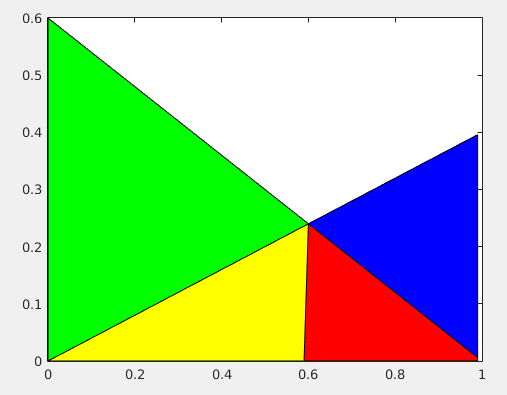
\includegraphics[scale=0.4]{Imgs/4-2.png}
\caption{Bayes decision boundary for proposed data in problem 4 when $p(w_1) = 0.4, p(w_2) = 0.6$}
\label{fig:4-2}
\end{figure}



The classification error is being calculated as a weighted sum of each misclassified point w.r.t. its probability. Therefore,
\begin{align*}
\epsilon = 0.4 * \epsilon_1 + 0.6 * \epsilon_2 = 0.4 * \int_0^0.6 0.4x dx + 0.6 * \int_0.6^1 0.6-0.6x dx = 0.0768
\end{align*}

\end{enumerate}

\begin{center}
\line(1,0){450}
\end{center}

%%%%%%%%%%%%%%%%%%%%%%%%%%%%%%%%%%%%%%%%%%%%%%%%%%%%%%%%%%%%%%%%%%%%%%%%%%%%%%%%%%%%%%%%%%%%%%%%%
\section{Problem 5}
Consider a two-category classification problem in two dimensions with:
\begin{align*}
p (X | W_1) \propto N ( 0 , I ), P ( X | W_2 ) \propto N (\svector{1}{0}, I) , P ( W_1 ) = P ( W_2 ) = 0.5 .
\end{align*}

\begin{enumerate}
\item Calculate the Bayes decision boundary.\\
As $\Sigma_1 = \Sigma_2 = \Sigma = I$, a one dimensional function $h(x)$ can be defined as bellow discriminating two classes linearly:
\begin{align*}
h(x) = (M_2 - M_1)^T\Sigma^{-1}X + \frac{1}{2}(M_1^T\Sigma^{-1}M_1 - M_2^T\Sigma^{-1}M_2)\gl ln \frac{P_1}{P_2}
\end{align*}
So the appropriate function is as follows:
\begin{align*}
&h(x) = \svector{1}{0}^TX + \frac{1}{2}( - \svector{1}{0}^T\svector{1}{0})\gl 0 \\
&\rightarrow h(x) = \svector{1}{0}^TX - \frac{1}{2}\gl 0 \\
\end{align*}

\begin{center}
\line(1,0){250}
\end{center}

%%%%%%%%%%%%%%%%%%%%%%%%%%%%%%%%%%%%%%%%%%%%
\item Calculate the Bhattacharyya error bound.\\
The Bhattacharyya error bound is in the form of following equation:
\begin{equation}
\epsilon = \sqrt{P(W_1)P(W_2)}e^{-\mu(0.5)}
\end{equation}
Where $\mu(0.5)$ for normal distribution is:
\begin{equation}
\mu(0.5) = \frac{1}{8} (M_2 - M_1)^T (\frac{\Sigma_1 + \Sigma_2}{2})^{-1} (M_2 - M_1) + \frac{1}{2} ln \frac{|\frac{\Sigma_1 + \Sigma_2}{2}|}{\sqrt{|\Sigma_1||\Sigma_2|}}
\end{equation}
Considering $\Sigma_1 = \Sigma_2 = I$ :
\begin{align*}
\mu(0.5) = \frac{1}{8} (M_2 - M_1)^T (M_2 - M_1) = \frac{1}{8}
\end{align*}
So:
\begin{align*}
\epsilon = \sqrt{P(W_1)P(W_2)}e^{-\mu(0.5)} = \frac{1}{2}e^{-\frac{1}{8}}
\end{align*}



\begin{center}
\line(1,0){250}
\end{center}

%%%%%%%%%%%%%%%%%%%%%%%%%%%%%%%%%%%%%%%%%%%%
\item Repeat the above for the same prior probabilities, but
\begin{align*}
p(X|W_1) \propto N(0, \smatrix{2}{0.5}{0.5}{2}), p(X|W_2) \propto N(\svector{1}{0}, \smatrix{5}{2}{2}{5})
\end{align*}
As $\Sigma_1 \neq \Sigma_2$, the one dimensional discriminant function $h(x)$ is formed as bellow:
\begin{align*}
&h(x) = \frac{1}{2} (x - M_1)^T \Sigma_1^{-1} (x - M_1) - \frac{1}{2} (x - M_2)^T \Sigma_2^{-1} (x - M_2) + \frac{1}{2} ln \frac{|\Sigma_1|}{|\Sigma_2|} \\
&\rightarrow h(x) = \frac{1}{3.75}x^T \smatrix{2}{-0.5}{-0.5}{2} x - \frac{1}{21}(x - \svector{1}{0})^T \smatrix{5}{-2}{-2}{5} (x - \svector{1}{0}) \\
&+ \frac{1}{2} ln \frac{|\smatrix{2}{0.5}{0.5}{2}|}{|\smatrix{5}{2}{2}{5}|} \\
&\rightarrow h(x) = \frac{1}{3.75}x^T \smatrix{2}{-0.5}{-0.5}{2} x - \frac{1}{21}(x - \svector{1}{0})^T \smatrix{5}{-2}{-2}{5} (x - \svector{1}{0}) + \frac{3.75}{42} \\
&\rightarrow h(x) = \frac{1}{3.75}x^T \smatrix{2}{-0.5}{-0.5}{2} x  - \frac{1}{21}(x^T\smatrix{5}{-2}{-2}{5}x -x^T\smatrix{5}{-2}{-2}{5}\svector{1}{0} \\
&- \svector{1}{0}^T\smatrix{5}{-2}{-2}{5}x - \svector{1}{0}^T\smatrix{5}{-2}{-2}{5}\svector{1}{0})\\
&\rightarrow h(x) = \frac{1}{78.75}x^T\smatrix{23.25}{-3}{-3}{23.25}x + \frac{1}{21}x^T\svector{5}{-2} + \frac{1}{21}\svector{5}{-2}^T x + \frac{1}{21}\svector{29}{-20}^TI + \frac{3.75}{42}\\
&\rightarrow h(x) = \frac{1}{78.75}x^T\smatrix{23.25}{-3}{-3}{23.25}x  + \frac{1}{21} \svector{10}{-4}^T x + \frac{21.75}{42}\\
\end{align*}
So the discriminant function is such as bellow:
\begin{align*}
 h(x) = \frac{1}{78.75}x^T\smatrix{23.25}{-3}{-3}{23.25}x  + \frac{1}{21} \svector{10}{-4}^T x + \frac{21.75}{42} .\gl 0
\end{align*}
The Bhattacharyya error bound is as bellow:
\begin{align*}
&\mu(0.5) = \frac{1}{8} (M_2 - M_1)^T (\frac{\Sigma_1 + \Sigma_2}{2})^{-1} (M_2 - M_1) + \frac{1}{2} ln \frac{|\frac{\Sigma_1 + \Sigma_2}{2}|}{\sqrt{|\Sigma_1||\Sigma_2|}} \\
&\mu(0.5) = \frac{1}{8} \svector{1}{0}^T (\frac{\smatrix{2}{0.5}{0.5}{2} + \smatrix{5}{2}{2}{5}}{2})^{-1} \svector{1}{0} + \frac{1}{2} ln \frac{|\frac{\smatrix{2}{0.5}{0.5}{2} + \smatrix{5}{2}{2}{5}}{2}|}{\sqrt{|\smatrix{2}{0.5}{0.5}{2}||\smatrix{5}{2}{2}{5}|}} \\
&\mu(0.5) = \frac{3.5}{85.5} + 0.4948 = 0.5357
\end{align*} 






\end{enumerate}







\begin{center}
\line(1,0){450}
\end{center}

%%%%%%%%%%%%%%%%%%%%%%%%%%%%%%%%%%%%%%%%%%%%%%%%%%%%%%%%%%%%%%%%%%%%%%%%%%%%%%%%%%%%%%%%%%%%%%%%%

\section{Problem 6}
Consider a two-category classification problem in two dimensions with $p(W_1 ) = p(W_2 )$,
assume that the class-conditional densities are Gaussian with mean $\mu_1$ and
co-variance $\Sigma_1$ under class 1, and mean $\mu_2$ and co-variance $\Sigma_2$ under class 2. Further, assume that $\mu_1 = \mu_2$. (Note that in the problem set, there was stated that $\mu0 = \mu1$, which I guessed that the correct form is $\mu_1 = \mu_2 $ rather than $\mu_0 = \mu_1$!)

\begin{align*}
\Sigma_1 = \smatrix{1}{0}{0}{4}, \Sigma_2 = \smatrix{4}{0}{0}{1}
\end{align*}

For the following case, draw contours of the level sets of the class conditional densities.
Also, draw the decision boundaries obtained using the Bayes optimal classifier in each case
and indicate the regions where the classifier will predict class 1 and where it will predict
class 2. \\

Calculating the Bayes decision boundary yields:
\begin{align*}
h(X) = \frac{1}{2}(X - \mu_1)^T\Sigma_1^{-1}(X - \mu_1) - \frac{1}{2} (X-\mu_2)^T\Sigma_2^{-1}(X-\mu_2) + \frac{1}{2} ln \frac{|\Sigma_1|}{|\Sigma_2|} .\gl ln \frac{P(W_1)}{P(W_2)}
\end{align*}
Considering the assumptions of the problem in addition to taking $\mu_1 = \mu_2 = \svector{0}{0}$ yields:
\begin{align*}
&h(X) = \frac{1}{2}X^T\smatrix{1}{0}{0}{4}^{-1}X - \frac{1}{2} X^T\smatrix{4}{0}{0}{1}^{-1}X + \frac{1}{2} ln \frac{|\smatrix{4}{0}{0}{1}|}{|\smatrix{1}{0}{0}{4}|} .\gl 0 \\
&\rightarrow h(X) = \frac{1}{8}X^T\smatrix{1}{0}{0}{4}X - \frac{1}{8}X^T\smatrix{4}{0}{0}{1}X\gl 0 \\
&\rightarrow h(X) = \frac{1}{8}\svector{1}{4}X^TX - \frac{1}{8}\svector{4}{1}X^TX .\gl 0 \\
&\rightarrow h(X) = \frac{3}{8}\svector{-1}{1}^T(X^TX) .\gl 0\\
&\rightarrow h(X) = \svector{-1}{1}^T(X^TX) .\gl 0\\
\end{align*}

A MATLAB script has been written to draw the required boundaries and regions. Figure \ref{fig:6-1} displays the result of this script.

\begin{figure}[h]
\centering
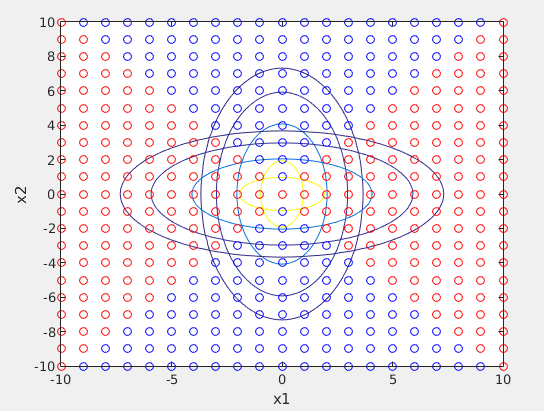
\includegraphics[scale=0.5]{Imgs/6.png}
\caption{Bayesian decision boundaries and class acceptance regions for data described in problem 6}
\label{fig:6-1}
\end{figure}

Contours of two classes are drawn in figure \ref{fig:6-1} and the acceptance region for each class has been displayed by coloured circles. The blue region is dedicated to the class $W_1$ and the red region is dedicated to class $W_1$.

\begin{center}
\line(1,0){450}
\end{center}

%%%%%%%%%%%%%%%%%%%%%%%%%%%%%%%%%%%%%%%%%%%%%%%%%%%%%%%%%%%%%%%%%%%%%%%%%%%%%%%%%%%%%%%%%%%%%%%%%

\section{Problem 7}
Consider the two-dimensional data points from two classes $W_1$ and $W_2$ below, and each of
them come from a Gaussian distribution $p ( x | W_k ) \propto N ( \mu_k , \Sigma_k )$. (Data table is not reported here)

\begin{enumerate}
\item What is the prior probability for each class, i.e. $p(W_1)$ and $p(W_2 )$ . \\

Assuming that the given table represents the distribution of original data, the probability of each class is proportional to the ratio of observed data from that class in the given small dataset. So, the $P(W_1) = \frac{6}{14} = 0.4286$ and therefore $P(W_2) = 1 - P(W_1) = 0.5714$.


\begin{center}
\line(1,0){250}
\end{center}

%%%%%%%%%%%%%%%%%%%%%%%%%%%%%%%%%%%%%%%%%%%
\item Calculate the mean and covariance matrix for each class. \\
Estimating sample mean and sample covariance matrix from data is according to the following equations:
\begin{equation}
\hat{\mu_i} = \frac{1}{N_i} \Sigma_{j=1}^{N_i} X_j
\end{equation}
For the covariance matrix $\Sigma^k = [\sigma_{ij}^k]$, in which $k$ denotes class number:
\begin{equation}
\hat{\sigma_{ij}^k} = \frac{1}{N_k - 1} \Sigma_{l=1}^{N_k} (x_{li} - \bar{x_i})(x_{lj} - \bar{x_j})
\end{equation}
So according to these equations:
\begin{equation}
\hat{\mu_1} = \svector{1.5}{1.3333}, \hat{\mu_2} = \svector{8.25}{8.625}
\end{equation}
and
\begin{equation}
\hat{\Sigma_1} = \smatrix{1.1}{1}{1}{1.8667}, \hat{\Sigma_2} = \smatrix{2.7857}{0.25}{0.25}{1.4107}
\end{equation}





\begin{center}
\line(1,0){250}
\end{center}

%%%%%%%%%%%%%%%%%%%%%%%%%%%%%%%%%%%%%%%%%%%
\item Derive the equation for the decision boundary that separates these two classes, and plot the boundary. (Hint: you may want to use the posterior probability)\\
Estimating class means and covariance matrices, the Bayesian decision boundary can be computed using the equations used in previous problems. 

\begin{align*}
&\frac{P(W_1|X)}{P(W_2|X)} .\gl \frac{P(W_2)}{P(W_1)} \\
&\frac{P(W_1|X)}{P(W_2|X)}  = \frac{P(X|W_1).P(W_1)}{P(X|W_2).P(W_2)} = \frac{N(\svector{1.5}{1.3333},\smatrix{1.1}{1}{1}{1.8667}).0.4286}{N(\svector{8.25}{8.625},\smatrix{2.7857}{0.25}{0.25}{1.4107}).0.5714} .\gl \frac{0.5714}{0.4286} 
\end{align*}
In which $N(\mu, \Sigma)$ represents the Gaussian normal function for each class and with corresponding mean vector and covariance matrix.


\begin{center}
\line(1,0){250}
\end{center}

%%%%%%%%%%%%%%%%%%%%%%%%%%%%%%%%%%%%%%%%%%%
\item Think of the case that the penalties for misclassification are different for the two classes (i.e. not zero-one loss), will it affect the decision boundary, and how? \\
Of course it will affect the decision boundary. Generally, the boundary is being tightened where the penalty of misclassification is less than other locations in favour of the locations in which the penalty of misclassification is larger. In other words, decision boundary will be adjusted in the way that make less misclassifications in the regions in which the penalty of misclassification is large, and prefer to make misclassifications in regions with less penalty.


\end{enumerate}


\begin{center}
\line(1,0){450}
\end{center}


%%%%%%%%%%%%%%%%%%%%%%%%%%%%%%%%%%%%%%%%%%%%%%%%%%%%%%%%%%%%%%%%%%%%%%%%%%%%%%%%%%%%%%%%%%%%%%%%%

\section{Problem 8}
Consider a classification problem with 2 classes and a single real-valued feature vector $X$. For class
1, $p(x | c_1 )$ is uniform $U(a, b)$ with $a = 2$ and $b = 4$. For class 2, $p(x|c_2 )$ is exponential with density $\lambda exp(-\lambda x)$ where $\lambda = 1$. Let $p(c_1) = p(c_2) = 0.5$.
\begin{enumerate}
\item Determine the location of the optimal decision regions
\begin{align*}
P(W_1|X)\gl P(W_2|X) &\rightarrow  P(X|W_1)P(W_1)\gl P(X|W_2)P(W_2) \\
&\rightarrow \frac{1}{4 - 2} .\gl e^{-x} \rightarrow -ln(2) .\gl -x \\
&\rightarrow x\gl ln(2)
\end{align*}
On the other hands, as $p(X|W_1) \propto U(2,4)$, data from class 1 are not defined in $R - [2,4]$. So there exists some implicit boundary conditions, $\forall X \in W_1, X \in [2,4]$. Comparing the probability densities in $X = ln(2)$,$X = 2$, $X = 4$ and everywhere $X > 4$, results choosing the region $[2, 4]$ as the acceptance region for class 1 and every other region as the acceptance region for class 2.\\
This above-mentioned fact, is obviously clear in the figure \ref{fig:8-1}, which represents the class densities and acceptance regions of classes.

\begin{center}
\line(1,0){250}
\end{center}

%%%%%%%%%%%%%%%%%%%%%%%%%%%%%%%%%%%%%%%%%%%
\item Draw a sketch of the two class densities multiplied by $P(c_1)$ and $P(c_2)$ respectively, as a
function of $x$, clearly showing the optimal decision boundary (or boundaries) \\
The figure \ref{fig:8-1}, displays class densities multiplied by class priors along side optimal decision boundaries extracted from section 1 of this current problem.\\
The yellow area, is acceptance region for class 1. As it is clear, the class 1 is not defined in $R-[2,4]$ and in its domain, its density multiplied by its prior is greater than that of class 2. So the yellow region is an optimal boundary for this class. On the other hands, in $R-[2,4]$, where class 1 is not defined, the optimal decision for data is obviously assigning that to class 2. The blue region in figure \ref{fig:8-1} displays optimal boundary for this class 2. The purple region displays the region of class 2 misclassifications.
\begin{figure}[h]
\centering
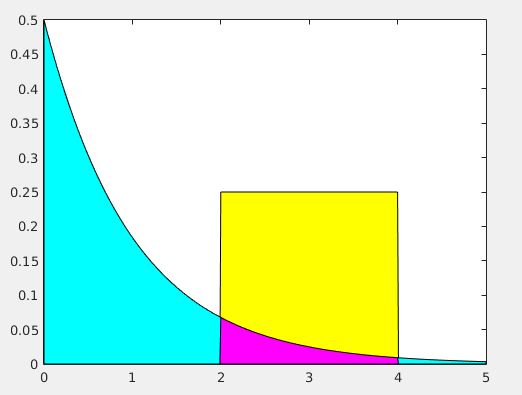
\includegraphics[scale=0.5]{Imgs/8-1.png}
\caption{Class densities multiplied by class priors for each class given their conditional distributions in problem 8 when $dom \> W_1 = [2,4]$}
\label{fig:8-1}
\end{figure}



\begin{center}
\line(1,0){250}
\end{center}

%%%%%%%%%%%%%%%%%%%%%%%%%%%%%%%%%%%%%%%%%%%
\item Compute the Bayes error rate for this problem within 3 decimal places of accuracy\\
The Bayes error rate is computable as bellow:
\begin{align*}
\epsilon = \int_2^4 0.5exp(-x)dx = -0.5exp(-4) + 0.5 exp(-2) = -0.5 * 0.018 + 0.5 * 0.135 = 0.058
\end{align*}

\begin{center}
\line(1,0){250}
\end{center}

%%%%%%%%%%%%%%%%%%%%%%%%%%%%%%%%%%%%%%%%%%%
\item Answer the questions above but now with $a = 2$ and $b = 22$.
Optimal decision boundary:
\begin{align*}
P(W_1|X)\gl P(W_2|X) &\rightarrow  P(X|W_1)P(W_1)\gl P(X|W_2)P(W_2) \\
&\rightarrow \frac{1}{22 - 2} .\gl e^{-x} \rightarrow -ln(20) .\gl -x \\
&\rightarrow x\gl ln(20) \rightarrow x\gl 2.9957
\end{align*}
\begin{figure}[h]
\centering
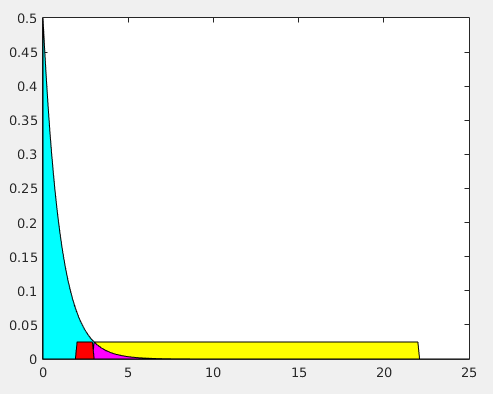
\includegraphics[scale=0.5]{Imgs/8-2.png}
\caption{Class densities multiplied by class priors for each class given their conditional distributions in problem 8 when $dom \> W_1 = [2,22]$}
\label{fig:8-2}
\end{figure}

Since the $x = 2.9957$ is in domain of class 1, the optimal point is itself and there is no need to compare it with boundary points of class 1. \\
Figure \ref{fig:8-2} displays the decision boundary for this properties. As it is clearly obvious, when $2 \leq X \leq ln(20)$, the optimum decision for $X$ is class 2 and when $ln(20) \leq X \leq 22$ the optimum decision is class 1 and after that when $X > 22$, as the class 1 is not defined there, the optimum decision is class 2 again.

Now, there is two types of error such that:
\begin{align*}
\epsilon = \in_2^{ln(20)} 0.5\frac{1}{22-2} dx + \int_{ln(20)}^22 0.5 exp(-x) dx = \frac{1}{40}(ln(20) - 2) + \frac{1}{2}(exp(-22) - \frac{1}{20})
\end{align*}

So, this is important to check the domain of each class in the cases in which the distribution of classes are finite and limited to a specific region. 

\end{enumerate}

\begin{center}
\line(1,0){450}
\end{center}

%%%%%%%%%%%%%%%%%%%%%%%%%%%%%%%%%%%%%%%%%%%%%%%%%%%%%%%%%%%%%%%%%%%%%%%%%%%%%%%%%%%%%%%%%%%%%%%%%

\section{Problem 9}
Consider a 2-class classification problem with d-dimensional real-valued inputs $x$, where the class-
conditional densities, $p ( x | c_1 )$ and $p ( x | c_2 )$ are multivariate Gaussian with different means $\mu_1$ and $\mu_2$ and a common covariance matrix $\Sigma$ , with class probabilities $P(c_1 )$ and $P(c_2 )$.
\begin{enumerate}
\item Write the discriminant functions for this problem in the form of $g_1 ( x ) = log p ( x | c_1 ) + log p ( c_1 )$ (same for $g_2 ( x )$ ). \\


\begin{center}
\line(1,0){250}
\end{center}

%%%%%%%%%%%%%%%%%%%%%%%%%%%%%%%%%%%%%%%%%%%

\item Prove that the optimal decision boundary, at $g ( x ) = g_1 ( x ) - g_2 ( x ) = 0$ , can be written in the form of a linear discriminant, $w^Tx + w_0 = 0$ , where $w$ is a d-dimensional weight vector and $w_0$ is a scalar, and clearly indicate what are $w$ and $w_0$ are in terms of
parameters of the classification model.\\
\end{enumerate}


\begin{center}
\line(1,0){450}
\end{center}

%%%%%%%%%%%%%%%%%%%%%%%%%%%%%%%%%%%%%%%%%%%%%%%%%%%%%%%%%%%%%%%%%%%%%%%%%%%%%%%%%%%%%%%%%%%%%%%%%

\section{Problem 10}
Consider the two-dimensional data points from two classes $W_1$ and $W_2$. (The data table is not reported here)

\begin{enumerate}
\item Determine and plot the optimal projection line in a single dimension using Fisher linear discriminant method. \\


\begin{center}
\line(1,0){250}
\end{center}

%%%%%%%%%%%%%%%%%%%%%%%%%%%%%%%%%%%%%%%%%%%
\item Show the mapping of the points to the line as well as the Bayes discriminant assuming a suitable distribution.\\



\end{enumerate}

\begin{center}
\line(1,0){450}
\end{center}

%%%%%%%%%%%%%%%%%%%%%%%%%%%%%%%%%%%%%%%%%%%%%%%%%%%%%%%%%%%%%%%%%%%%%%%%%%%%%%%%%%%%%%%%%%%%%%%%%

\section{Problem 11}
[Computer Experiment] In this problem, you will be classifying the “Iris” dataset from the UCI Machine Learning Repository. The original data describes 3 classes of Iris flowers and contains various measurements about them: 
\begin{enumerate}
\item sepal length in cm 
\item sepal width in cm
\item petal length in cm 
\item petal width in cm
\end{enumerate}
To make things a little easier, we left out one of the flower types and only included the “Iris Setosa” (class 0) and “Iris Versicolor” (class 1). There are two data files for this assignment, a training data set (70 data items) and a test data set (30 data items). \\

Every line in each file describes one data item; the 5 numbers in each row contain the 4 measurements in above order plus the class label. Use only the second measurement (sepal width) for classification and ignore all others.


\begin{enumerate}
\item Load the training data. Compute a feature histogram for each class (see histc and bar in Matlab), using edges between the bins at 0.2 intervals between 1 and 5; i.e. 1 : 0.2 : 5. Show the histograms either in two figures using subplot in Matlab, and make sure both plots have the same x-axis range.\\

\begin{center}
\line(1,0){250}
\end{center}

%%%%%%%%%%%%%%%%%%%%%%%%%%%%%%%%%%%%%%%%%%%
\item Estimate the class priors from the training data. Report the prior probabilities of a flower being an “Iris Setosa” or being an “Iris Versicolor”.\\

\begin{center}
\line(1,0){250}
\end{center}

%%%%%%%%%%%%%%%%%%%%%%%%%%%%%%%%%%%%%%%%%%%
\item Assume that we can model the class-conditional probability density of each class using a univariate Gaussian (remember to only use the sepal width). What are the mean and variance of both class-conditional densities?\\

\begin{center}
\line(1,0){250}
\end{center}

%%%%%%%%%%%%%%%%%%%%%%%%%%%%%%%%%%%%%%%%%%%
\item Plot the estimated class-conditional densities in a single diagram. Make a second figure plotting the class posteriors for both classes. Write down the equation you used to compute the class posteriors .\\

\begin{center}
\line(1,0){250}
\end{center}

%%%%%%%%%%%%%%%%%%%%%%%%%%%%%%%%%%%%%%%%%%%
\item Compute the Bayes classification of the training data. How many “Setosas” do you mistakenly classify as “Versicolor” and how many “Versicolors” do you mistakenly classify as “Setosa”? What is the overall training error (i.e. percentage of incorrectly classified training data items)?\\

\begin{center}
\line(1,0){250}
\end{center}

%%%%%%%%%%%%%%%%%%%%%%%%%%%%%%%%%%%%%%%%%%%
\item Now classify the test data. How many “Setosas” do you mistakenly classify as “Versicolor” and how many “Versicolors” do you mistakenly classify as “Setosa”? Report the number of cases that are incorrectly classified as above as well as the test error.\\

\end{enumerate}

\begin{center}
\line(1,0){450}
\end{center}

%%%%%%%%%%%%%%%%%%%%%%%%%%%%%%%%%%%%%%%%%%%%%%%%%%%%%%%%%%%%%%%%%%%%%%%%%%%%%%%%%%%%%%%%%%%%%%%%%





























\bibliographystyle{plain}
\bibliography{biblist}

\end{document}